\documentclass{article}
\usepackage{tikz}

\begin{document}

\begin{figure}[h]
    \centering
    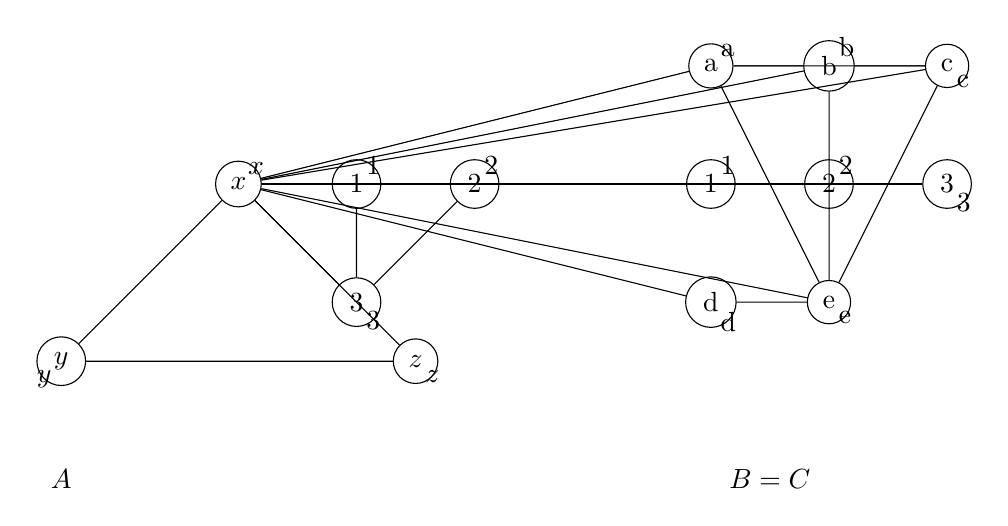
\begin{tikzpicture}[scale=1.5]

        % Define nodes
        \node (x) at (0, 0) [circle, draw] {$x$};
        \node (y) at (-1.5, -1.5) [circle, draw] {$y$};
        \node (z) at (1.5, -1.5) [circle, draw] {$z$};

        % Draw edges
        \draw (x) -- (y);
        \draw (x) -- (z);
        \draw (y) -- (z);

        % Label nodes
        \node at (x) [above right] {$x$};
        \node at (y) [below left] {$y$};
        \node at (z) [below right] {$z$};

        % Subgraph A
        \node (a1) at (1, 0) [circle, draw] {1};
        \node (a2) at (2, 0) [circle, draw] {2};
        \node (a3) at (1, -1) [circle, draw] {3};

        \draw (x) -- (a1);
        \draw (x) -- (a2);
        \draw (x) -- (a3);
        \draw (a1) -- (a2);
        \draw (a2) -- (a3);
        \draw (a3) -- (a1);

        % Label subgraph A
        \node at (a1) [above right] {1};
        \node at (a2) [above right] {2};
        \node at (a3) [below right] {3};

        % Subgraph B = C
        \node (b1) at (4, 0) [circle, draw] {1};
        \node (b2) at (5, 0) [circle, draw] {2};
        \node (b3) at (6, 0) [circle, draw] {3};

        \node (c1) at (4, 1) [circle, draw] {a};
        \node (c2) at (5, 1) [circle, draw] {b};
        \node (c3) at (6, 1) [circle, draw] {c};

        \node (d1) at (4, -1) [circle, draw] {d};
        \node (d2) at (5, -1) [circle, draw] {e};

        \draw (x) -- (b1);
        \draw (x) -- (b2);
        \draw (x) -- (b3);
        \draw (x) -- (c1);
        \draw (x) -- (c2);
        \draw (x) -- (c3);
        \draw (x) -- (d1);
        \draw (x) -- (d2);

        \draw (b1) -- (b2);
        \draw (b2) -- (b3);
        \draw (b3) -- (b1);

        \draw (c1) -- (c2);
        \draw (c2) -- (c3);
        \draw (c3) -- (c1);

        \draw (d1) -- (d2);
        \draw (d2) -- (c1);
        \draw (d2) -- (c2);
        \draw (d2) -- (c3);

        % Label subgraph B = C
        \node at (b1) [above right] {1};
        \node at (b2) [above right] {2};
        \node at (b3) [below right] {3};

        \node at (c1) [above right] {a};
        \node at (c2) [above right] {b};
        \node at (c3) [below right] {c};

        \node at (d1) [below right] {d};
        \node at (d2) [below right] {e};

        % Labels for subgraphs
        \node at (-1.5, -2.5) {$A$};
        \node at (4.5, -2.5) {$B = C$};

    \end{tikzpicture}
\end{figure}

\end{document}